\subsection{Measurement Integrity}
\label{sec:integrity-results}

\emph{Competition record.} The competition record contains 90\,min of
reports from the eight PMUs (161{,}379 reports per PMU). Its labels mark four
dropout events of PMU~29 (\IntMissReports{} reports) and three
corrupted-data episodes at PMUs~2 and~39. A separate class~6 label
composes a missing PMU with the generation event at bus~2 and is counted
as an additional event by the competition scorer; the integrity monitor
still sees the same missing frames. We applied the two parity relations of
Section~\ref{sec:integrity-theory} and the frame flag. Separate voltage
and current noise scales for each PMU were estimated from the first 3\,s
of the record; there was no training and labels were used only for scoring.
Table~\ref{tab:integrity-raw} and Fig.~\ref{fig:integrity} give the
results. All \IntMissTot{} dropouts and all \IntCorrTot{} corruptions were
diagnosed at their first report and located at the correct PMU. The
corrupted phase was identified in \IntPhaseOK/\IntCorrTot{} episodes. The
third corruption is intermittent, with a median step below 1\%, and is
flagged in 15 of its 32 reports.
\begin{table}[t]\centering\small
\caption{Labeled integrity episodes of the competition record and their diagnosis. Delay is in reports after the first labeled report; ``flagged'' counts diagnosed reports within the episode; phase is identified (labeled-data phase). Every episode was located at the correct PMU.}
\label{tab:integrity-raw}
\footnotesize\setlength{\tabcolsep}{3.5pt}\begin{tabular}{@{}llrrrrl@{}}\toprule
Type & PMU & Start (s) & Length (s) & Delay & Flagged & Phase\\\midrule
Corrupted & 2 & 3.3 & 0.73 & 0 & 22/22 & C (C)\\
Corrupted & 39 & 334.4 & 0.77 & 0 & 23/23 & A (A)\\
Corrupted & 39 & 336.5 & 1.07 & 0 & 15/32 & A (A)\\
Missing & 29 & 536.6 & 27.07 & 0 & 812/812 & --\\
Missing & 29 & 614.3 & 29.10 & 0 & 873/873 & --\\
Missing & 29 & 2584.7 & 191.43 & 0 & 5743/5743 & --\\
Missing & 29 & 2935.8 & 59.07 & 0 & 1772/1772 & --\\
\bottomrule\end{tabular}\end{table}


\begin{figure*}[t]\centering
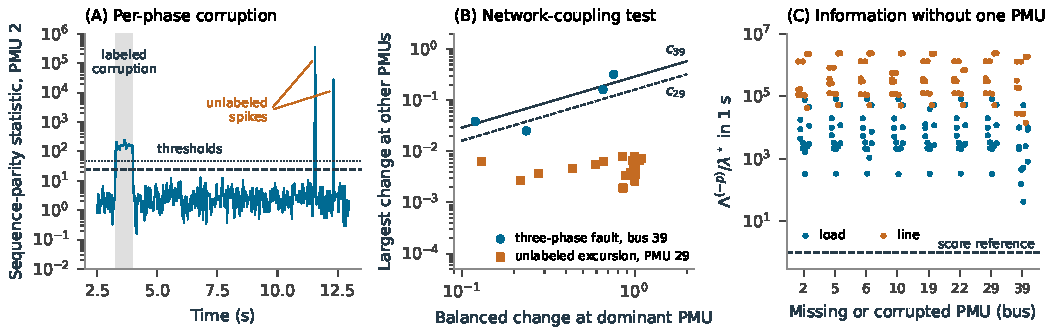
\includegraphics[width=.97\textwidth]{figures/generated/integrity.pdf}
\caption{Measurement integrity from network physics. (A) Sequence-parity statistic of PMU~2 on the competition record: a labeled single-phase corruption and two unlabeled single-report current spikes; dashed and dotted lines are the prespecified and variance-inflated thresholds. (B) Balanced voltage changes larger than 10\%: reports of the three-phase fault at bus~39 lie near the network-coupling bound $c_{39}$ of \eqref{eq:coupling-bound} and above the quarter of it used by the test, whereas the unlabeled collapse at PMU~29 lies two orders of magnitude below $c_{29}$. (C) Information for each held-out simulated intervention when one PMU is missing or corrupted (Proposition~\ref{prop:integrity}), relative to the idealized score reference $\lambda^\star$, under independent component noise with standard deviation $0.0005$ (relative magnitudes and radian angles).}
\label{fig:integrity}\end{figure*}

The three-phase fault at bus~39 produces negative-sequence transients at
seven PMUs at once. Its four reports with a balanced change above 10\% lie
between 0.37 and 1.5 times the coupling bound, above the quarter of the
bound used by the test (Fig.~\ref{fig:integrity}B). The lowest ratio occurs
at the first report, where the phasor estimation window has reached the
faulted bus before the others. The fault is therefore recognized as
physical, and parity is suspended while it lasts.
The threshold $q>\IntTau$ is the nominal $10^{-9}$ tail point for one
idealized sequence statistic. The implemented report statistic is the
maximum of voltage and current, so its ideal marginal tail is at most
$2\times10^{-9}$ before accounting for scale estimation. Across the eight
PMUs this record contains about 1.29 million monitored PMU-reports, for an
ideal-model expectation below 0.0026 exceedances; we observe
\IntNoiseExceed{} isolated single-report values with
$\IntTau<q<\IntTauInf$ (about $7.4\times10^3$ times that reference
expectation). This
shows that the nominal Gaussian tail model does not calibrate this record.
Doubling the assumed noise variance ($q>\IntTauInf$) removes these
exceedances and keeps every labeled episode. This operating point was
chosen after inspection and is not an independently calibrated FAR.
Two single-report flags remain at switching instants: the line opening,
and the generation change at the bus of PMU~2. This gives
\IntSwitchRate{} false alarms per minute.

The monitor also flags \IntUnlabeled{} incidents that the labels leave as
normal operation. Four are single-report current spikes: 2{,}485\,A and
53\,A in phase~B of PMU~2, against about 585\,A, and 702\,A and 710\,A in
phase~A of PMU~39, against 245\,A. One is a corrupted frame just before a
dropout of PMU~29. The last is a 2.2-s interval after a reconnection in
which all three voltage magnitudes of PMU~29 fall to zero, some of them
negative, while every other PMU changes by less than 1\%. A bolted fault
at bus~29 would change another PMU by at least $c_{29}=\IntCouplingTwentyNine$
times the change at PMU~29. The excursions are inconsistent with the tested single-fault model.
We report them as unlabelled integrity candidates, separately from false alarms.

\emph{Physical bank under integrity events.} The physical bank cannot run on
the competition record. Its startup test rejects the first 10\,s of the
record: the ROCOF channels of two PMUs are constant or quantized, and the
angle reference drifts by 0.31\,deg/s with respect to the calibrated
model. We therefore inserted the competition's integrity events into the
four held-out simulated event records and two normal records of
the noise-stress study, and ran the bank with its code unchanged.
\emph{Corruption}: we added \IntSimCorr{} 0.75-s steps of $+2.4\%$ or
$-2.6\%$ to the positive-sequence voltage magnitude of one PMU, the
positive-sequence equivalent of the two labeled corruptions. They rotate
over all PMUs, and four fall inside interventions. \IntSimCorrAlarm{} of
them produced a physical alarm, and the timely attributions were unchanged
(\IntSimCorrLoad/12 loads, \IntSimCorrLine/12 lines).
\emph{Missing data}: one PMU was removed for 27\,s, starting 2\,s before an
intervention, and replaced by its last valid report, the imputation
suggested by the competition guide. Of the \IntSimMissInside{}
interventions that began while a PMU was missing, the bank attributed
\IntSimMissInsideTimely{} in time, and the dropouts caused \IntSimMissExtras{}
unmatched alarms on the event records. \IntSimMissText{}

Together these results separate the integrity mechanisms from the
physical ones. Missing data are identified exactly and leave ample
nominal signature separation, but the implemented bank
cannot use it when fed held values; it needs the availability-switched
operator. Corruption is flagged by departures from the assumed measurement and network model. It did not mislead the bank in simulation, and on the
competition record it revealed incidents that the labels miss.
